\documentclass{beamer}
\usetheme{Rochester}
\usepackage{tcolorbox}
\tcbuselibrary{listings}
\usepackage{inconsolata}

\geometry{paperwidth = 4.75in, paperheight = 4.75in}

% Custom U of C color palette
\definecolor{ucMaroon}{RGB}{128,0,0}
\definecolor{ucDarkGray}{RGB}{118,118,118}
\definecolor{ucLightGray}{RGB}{214,214,206}

\setbeamercolor{block title}{fg=white,bg=ucMaroon}
\setbeamercolor{block title alerted}{use=alerted text,fg=white,bg=alerted text.fg}
\setbeamercolor{block title example}{use=example text,fg=white,bg=example text.fg}
\setbeamercolor{block body}{parent=normal text,use=block title,bg=ucLightGray}
\setbeamercolor{block body alerted}{parent=normal text,use=block title alerted,bg=block title alerted.bg}
\setbeamercolor{block body example}{parent=normal text,use=block title example,bg=block title example.bg}

\setbeamercolor{palette primary}{fg=white,bg=ucMaroon}
\setbeamercolor{palette secondary}{fg=white,bg=ucLightGray}
\setbeamercolor{palette tertiary}{fg=white,bg=ucDarkGray}
\setbeamercolor{palette quaternary}{fg=white,bg=black}

\setbeamercolor{sidebar}{bg=ucMaroon}

\setbeamercolor{palette sidebar primary}{fg=ucMaroon}
\setbeamercolor{palette sidebar secondary}{fg=white}
\setbeamercolor{palette sidebar tertiary}{fg=ucMaroon}
\setbeamercolor{palette sidebar quaternary}{fg=white}

\setbeamercolor{titlelike}{parent=palette primary}
\setbeamercolor{itemize item}{fg=ucMaroon}

% Code block formatting. Fragile frames needed for these to work.
\newtcblisting{gitCommand}{
  colframe=black,
  colback=ucLightGray,
  boxrule=1pt,
  arc=2pt,
  left=6pt,
  right=6pt,
  top=6pt,
  bottom=6pt,
  before=\vspace{6pt},
  boxsep=0pt,
  listing only,
  hbox
}


\title{Intermediate Git}
\subtitle{Day 1: Understanding Git's Worldview}
\author{Raman A.~Shah}
\date{}

\begin{document}

%% Title
\begin{frame}[plain]
  \titlepage
  \footnotesize{Copyright (c) 2015 by Raman A.~Shah.\\
  \href{https://creativecommons.org/licenses/by-nc-sa/3.0/legalcode}
       {Creative Commons BY-NC-SA 3.0 Unported}.\\
   \href{https://github.com/ramanshah/intermediate\_git}
        {https://github.com/ramanshah/intermediate\_git}}

\end{frame}

%% Have students do initial config if they haven't already.
\begin{frame}[fragile]{Some initial configuration}
  \begin{gitCommand}git config --list\end{gitCommand}

  If your user name and email are not set:

  \begin{gitCommand}
git config --global user.name \
  "Raman A. Shah"
git config --global user.email \
  "raman@uchicago.edu"
  \end{gitCommand}

  If you don't like \texttt{vim} firing up in the middle of doing Git stuff:

  \begin{gitCommand}git config --global core.editor "nano"\end{gitCommand}

\end{frame}

%% Git is...
%% ...a distributed version control system.
\begin{frame}{Git is\ldots}
  \huge {
    \begin{tabbing}
      \ldots a \= distributed \\
      \> version control \\
      \> \color{ucMaroon}{system}\color{black}{.}
    \end{tabbing}
  }
\end{frame}

\begin{frame}{Git is\ldots}
  \huge {
    \begin{tabbing}
      \ldots a \= distributed \\
      \> \color{ucMaroon}{version control} \\
      \> system.
    \end{tabbing}
  }
\end{frame}

\begin{frame}{Git is\ldots}
  \huge {
    \begin{tabbing}
      \ldots a \= \color{ucMaroon}{distributed} \\
      \> version control \\
      \> system.
    \end{tabbing}
  }
\end{frame}

\begin{frame}{Git is\ldots}
  \begin{figure}
    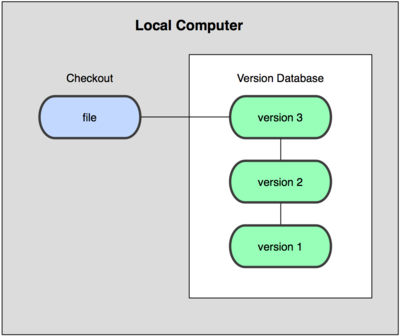
\includegraphics[scale=0.8]{18333fig0101-tn.png}
    \\ Local version control (\emph{e.g.}, \texttt{rcs}).
  \end{figure}
  \footnotesize{Scott Chacon,
    \emph{Pro Git},
    Fig.~1-1.
    \href{https://creativecommons.org/licenses/by-nc-sa/3.0/legalcode}{CC-BY-NC-SA}.
    \href{https://progit.org/}{https://progit.org/}}

\end{frame}

\begin{frame}{Git is\ldots}
  \begin{figure}
    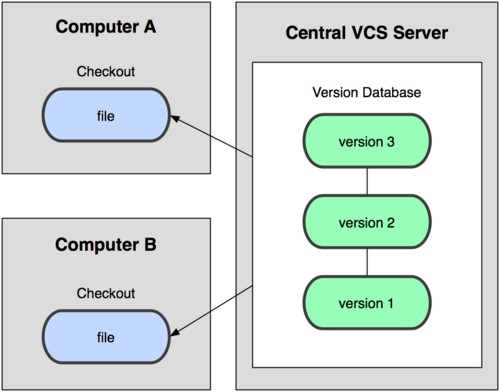
\includegraphics[scale=0.8]{18333fig0102-tn.png}
    \\ Centralized version control (\emph{e.g.}, CVS, Subversion (SVN), Perforce).
  \end{figure}
  \footnotesize{Scott Chacon,
    \emph{Pro Git},
    Fig.~1-2.
    \href{https://creativecommons.org/licenses/by-nc-sa/3.0/legalcode}{CC-BY-NC-SA}.
    \href{https://progit.org/}{https://progit.org/}}

\end{frame}

\begin{frame}{Git is\ldots}
  \begin{figure}
    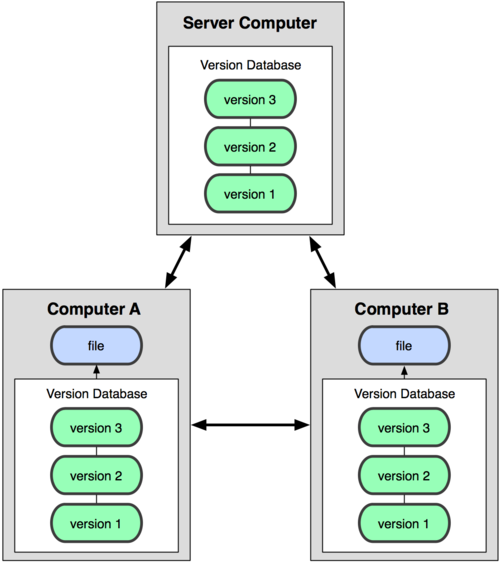
\includegraphics[scale=0.8]{18333fig0103-tn.png}
    \\ Distributed version control (\emph{e.g.}, \texttt{rcs}).
  \end{figure}
  \footnotesize{Scott Chacon,
    \emph{Pro Git},
    Fig.~1-3.
    \href{https://creativecommons.org/licenses/by-nc-sa/3.0/legalcode}{CC-BY-NC-SA}.
    \href{https://progit.org/}{https://progit.org/}}

\end{frame}

%% Git is...
%% ...a great way to collaborate on projects consisting of many code or text files.
\begin{frame}{Git is\ldots}
  \hangindent=26pt \huge {
  \ldots a great way to collaborate on projects consisting of
    many code or text files.
  }
\end{frame}

%% Git is...
%% ...meant for perfecting (software) products.
\begin{frame}{Git is\ldots}
  \hangindent=26pt \huge {
  \ldots meant for perfecting (software) \emph{products}.
  }
\end{frame}

%% Git is...
%% ...a content-addressable filesystem.
\begin{frame}{Git is\ldots}
  \hangindent=26pt \huge {
  \ldots a content addressable filesystem.
  }
\end{frame}

%% Exploring repository internals
\begin{frame}[fragile]{Exploring repository internals}
  From a place where you wouldn't mind a new subdirectory:

  \begin{gitCommand}git clone [URL]\end{gitCommand}

  \begin{gitCommand}cd [repo name]\end{gitCommand}

  \begin{gitCommand}git status\end{gitCommand}

\end{frame}

\begin{frame}[fragile]{Exploring repository internals}
  Explore the contents of \texttt{.git} and \texttt{.gitignore}. To
  list a directory's contents including hidden ``dotfiles'':

  \begin{gitCommand}ls -al\end{gitCommand}

  To write out the contents of a file to the terminal:

  \begin{gitCommand}cat [filename]\end{gitCommand}

\end{frame}

%% Git is...
%% ...safe because it tracks every single bit in your files and
%% commits with hash functions.
\begin{frame}{Git is\ldots}
  \hangindent=26pt \huge {
  \ldots safe because it tracks every single bit in your files and commits with
  hash functions.
  }
\end{frame}

%% Hash functions
\begin{frame}[fragile]{Hashes (checksums)}
  \begin{figure}
    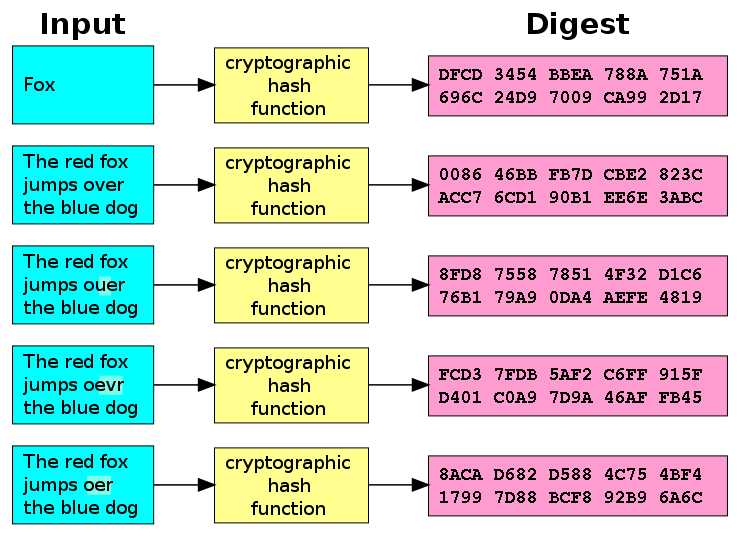
\includegraphics[scale=0.25]{hash_functions.png}
    \\ SHA-1 maps a file or text to a 160-bit value in a scrambly way.
  \end{figure}

  \begin{gitCommand}echo 'a' | sha1sum\end{gitCommand}

  \begin{gitCommand}sha1sum standup_snitch.py\end{gitCommand}
\end{frame}

%% Content addressability
\begin{frame}{Content addressability}
  \begin{figure}
    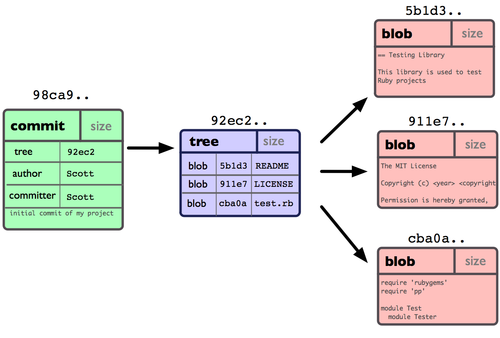
\includegraphics[scale=0.85]{18333fig0301-tn.png}
    \\ Content is snapshotted at the blob, tree, and commit levels.
  \end{figure}
  \footnotesize{Scott Chacon,
    \emph{Pro Git},
    Fig.~3-1.
    \href{https://creativecommons.org/licenses/by-nc-sa/3.0/legalcode}{CC-BY-NC-SA}.
    \href{https://progit.org/}{https://progit.org/}}
\end{frame}

%% Git is...
%% ...fast because it stores a (compressed) copy of every version of
%% every file locally.
\begin{frame}{Git is\ldots}
  \hangindent=26pt \huge {
  \ldots fast because it stores a (compressed) copy of every version
  of every file locally.
  }
\end{frame}

\begin{frame}{Git is\ldots}
  \begin{figure}
    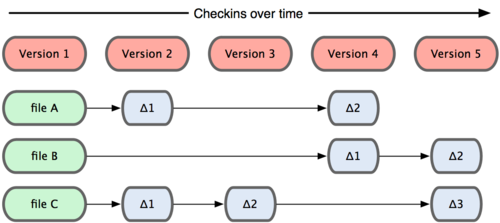
\includegraphics[scale=0.8]{18333fig0104-tn.png}
    \\ Other version control systems require calculating versions of a file with diffs.
  \end{figure}
  \footnotesize{Scott Chacon,
    \emph{Pro Git},
    Fig.~1-4.
    \href{https://creativecommons.org/licenses/by-nc-sa/3.0/legalcode}{CC-BY-NC-SA}.
    \href{https://progit.org/}{https://progit.org/}}

\end{frame}

\begin{frame}{Git is\ldots}
  \begin{figure}
    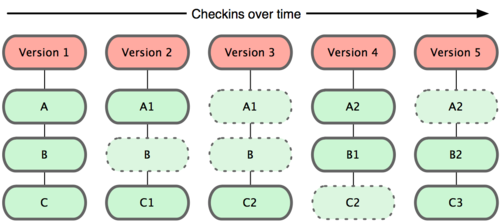
\includegraphics[scale=0.8]{18333fig0105-tn.png}
    \\ Git just stores all (unique) versions.
  \end{figure}
  \footnotesize{Scott Chacon,
    \emph{Pro Git},
    Fig.~1-5.
    \href{https://creativecommons.org/licenses/by-nc-sa/3.0/legalcode}{CC-BY-NC-SA}.
    \href{https://progit.org/}{https://progit.org/}}

\end{frame}

%% Git is...
%% ...hard because efficiently managing version control and collaboration is hard.
\begin{frame}{Git is\ldots}
  \hangindent=26pt \huge {
  \ldots hard because efficiently managing version control and collaboration is
  hard.*
  }
\end{frame}

%% Playing with the past
\begin{frame}[fragile]{Playing with the Past}
  \begin{gitCommand}git log\end{gitCommand}
  \begin{gitCommand}git diff\end{gitCommand}
  \begin{gitCommand}git blame\end{gitCommand}
  \begin{gitCommand}git show\end{gitCommand}
  \begin{gitCommand}git checkout\end{gitCommand}
\end{frame}

%% Reviewing history: git log
\begin{frame}[fragile]{Reviewing history: git log}
  Default log; type \texttt{q} to quit:

  \begin{gitCommand}git log\end{gitCommand}

  Limit the output to just the two most recent commits, and show some extra
  statistics:

  \begin{gitCommand}git log --stat -2\end{gitCommand}

  A single line of output per commit:

  \begin{gitCommand}git log --oneline\end{gitCommand}

  And much, much more.

  \begin{gitCommand}git help log\end{gitCommand}
\end{frame}

%% Finding changes: git diff
\begin{frame}[fragile]{Finding changes: git diff}

  \texttt{HEAD} is a ``You Are Here'' pointer. Tilde notation lets us
  walk back in history.

  \begin{gitCommand}git diff HEAD~\end{gitCommand}

  Equivalently:

  \begin{gitCommand}git diff HEAD~1\end{gitCommand}

  From three commits ago to one commit ago:

  \begin{gitCommand}git diff HEAD~3 HEAD~1\end{gitCommand}

  You can specify with hashes, and single out specific files:

  \begin{gitCommand}
git diff [older hash] [newer hash] \
  [path]
  \end{gitCommand}

\end{frame}

%% Finding authors: git blame
\begin{frame}[fragile]{Finding authors: git blame}

  \begin{gitCommand}git blame [path]\end{gitCommand}

  Good for:

  \begin{itemize}
    \item Blaming people for mistakes (as advertised)
    \item Figuring out whom to ask for guidance or code review
  \end{itemize}

\end{frame}

%% Seeing old versions: git show
\begin{frame}[fragile]{Seeing old versions: git show}
  To see the contents of an old version of a single file on the screen:

  \begin{gitCommand}git show [commit]:[path]\end{gitCommand}

  You can redirect it to a file outside of the repo to recover an old version.
\end{frame}

%% Time travel: git checkout
\begin{frame}[fragile]{Time travel: git checkout}
  Rewrite the contents of the directory to reflect the repository one commit
  ago:

  \begin{gitCommand}git checkout HEAD~1\end{gitCommand}

  Rewrite them back:

  \begin{gitCommand}git checkout master\end{gitCommand}

\end{frame}

%% Git is not...
%% ...a great system for documenting (experimental) projects.
\begin{frame}{Git is not\ldots}
  \hangindent=26pt \huge {
  \ldots a great system for documenting (experimental) \emph{projects}.
  }
\end{frame}

%% Git is not...
%% ...ideal for storing bulky data.
\begin{frame}{Git is not\ldots}
  \hangindent=26pt \huge {
  \ldots ideal for storing bulky data.*
  }
\end{frame}

%% Git is not...
%% ...quite as helpful for binary files as for text files.
\begin{frame}{Git is not\ldots}
  \hangindent=26pt \huge {
  \ldots quite as helpful for binary files as for text files.
  }
\end{frame}

%% Git is not...
%% ...a silver bullet for collaborating on written works.
\begin{frame}{Git is not\ldots}
  \hangindent=26pt \huge {
  \ldots a silver bullet for collaborating on written works.
  }
\end{frame}

%% Ph.D. comic
\begin{frame}{Git is\ldots}
  \begin{figure}
    
\includegraphics[scale=0.5]{phd101212s.png}
    \\ \ldots better than many alternatives!
  \end{figure}
  \footnotesize{``Piled Higher and Deeper'' by Jorge Cham\\
    www.phdcomics.com}

\end{frame}

\end{document}
